


%%%%%%%%%%%%%%%%%%%%%%%%%%%%%%%%%%%%%%%%%%%%%%%%%%%%%%%%%%%%%%%%
%%%%%%%%%%%  see documentation for information about  %%%%%%%%%%
%%%%%%%%%%%  the options (11pt, defaultstyle, etc.)   %%%%%%%%%%
%%%%%%%%%%%%%%%%%%%%%%%%%%%%%%%%%%%%%%%%%%%%%%%%%%%%%%%%%%%%%%%%
%%%%  http://www.Colorado.EDU/ITS/docs/latex/ThesisClass/  %%%%%
%%%%%%%%%%%%%%%%%%%%%%%%%%%%%%%%%%%%%%%%%%%%%%%%%%%%%%%%%%%%%%%%

%	\documentclass[defaultstyle]{thesis}
%	\documentclass[typewriterstyle]{thesis}
% 	\documentclass[modernstyle]{thesis}
%	\documentclass[modernstyle,12pt]{thesis}
	\documentclass[modernstyle,12pt]{seminar}

% 	\documentclass[modernstyle,11pt]{thesis}
% 	\documentclass[defaultstyle,12pt]{thesis}


%%%%%%%%%%%%%%%%%%%%%%%%%%%%%%%%%%%%%%%%%%%%%%%%%%%%%%%%%%%%%%%%
%%%%%%%%%%%    load any packages which are needed    %%%%%%%%%%%
%%%%%%%%%%%%%%%%%%%%%%%%%%%%%%%%%%%%%%%%%%%%%%%%%%%%%%%%%%%%%%%%



\usepackage{graphics}
\usepackage{graphicx}
\usepackage{latexsym}		% to get LASY symbols
\usepackage{epsfig}		% to insert PostScript figures
\usepackage{rotating}		% for sideways tables/figures
\usepackage{eufrak}




%%%%%%%%%%%%%%%%%%%%%%%%%%%%%%%%%%%%%%%%%%%%%%%%%%%%%%%%%%%%%%%%
%%%%%%%%%%%%       all the preamble material:       %%%%%%%%%%%%
%%%%%%%%%%%%%%%%%%%%%%%%%%%%%%%%%%%%%%%%%%%%%%%%%%%%%%%%%%%%%%%%


%%%%%%%%%%%% Parameters To be populated by the author START %%%%%%%%%%%%%
\title{PC Control Using Android}
\author{Amrutha}{K. V.}

%\authorTwo{Neethu C. P.}
%\authorThree{Sreelakshmi T. G.}
%\authorFour{Thahsin P.}
% \authorFive{Fasna P.P.}

\advisor{}{Mr Sherikh K. K.}			%  #1 {title}

\rollnum{14BCS12163}                                  % roll number
%\rollnumTwo{14BCS12164}                                  % roll number 2
%\rollnumThree{14BCS12165}                                  % roll number 3
%\rollnumFour{13BCS11154}                                  % roll number 4
% \rollnumFive{MCS09303314}                                  % roll number 5

\degreeyear{2015-16}                                     % academic year
%%%%%%%%%%%% Parameters To be populated by the author END %%%%%%%%%%%%%



%\otherdegrees{B.A., North Dakota State University, 1994 \\
%	      M.S., University of Reno, 1997}

\degree{\Large {$\mathfrak {Bachelor\; of\; Technology}$}}		%  #1 {long descr.}
	{M.Tech., Computer Science and Engineering}		%  #2 {short descr.}

\dept{Department of}			%  #1 {designation}
	{Computer Science and Engineering}		%  #2 {name}




\reader{Dr. Mredhula L.}		%  2nd person to sign thesis
%\readerThree{Ms.~Thora Nea}		%  3rd person to sign thesis
% \readerFour{Mr.~Alfred Remington}	%  4rd person to sign thesis


\inst{MES College of Engineering, Kuttippuram}                   % institution

%\deg{Master of Technology}		             %  degree name (in certificate)
\course{Computer Science and Engineering}    %  course name


%%%%%%%%%%%% Add your abstract here! START %%%%%%%%%%%%%

\abstract{  \OnePageChapter	% one page only ??
	�PC Control� is a mobile application software for parents to monitor and control their child PC remotely. It enables one to monitor the remote machines desktop and thus control it with their android touch pointer. It can be used with Microsoft Windows to perform real time remote system control and administration tasks through different network environments. This application software requires a TCP/IP connection between the server and the client, which works  either in LAN's or in WAN's; even on internet if one provides a IP address for their machine. When the connection between a client and a server is first established, the server begins by requesting authentication from the client using an authentication, which typically results in the user being prompted for a user name and password at the client end. It does, however, provide the primary user of a PC with remote access to their desktop. There will be an option to send messages to the server machine; these messages will be notified on the server screen. In addition to the control through desktop; there will be short cuts (i.e. single click actions) for power options.}
}
%%%%%%%%%%%% Add your abstract here! END %%%%%%%%%%%%%

%%%%%%%%%%%% Add your acknowledgements here! START %%%%%%%%%%%%%
\acknowledgements{	\OnePageChapter	% *MUST* BE ONLY ONE PAGE!
	First of all I wish to thank God Almighty for His blessings that made our work a success. 
	
	I am grateful to Dr.V.H.Abdul Salam, Principal, MES College of Engineering, Kuttippuram, for providing the right ambiance to do this project. I would like to extend our sincere gratitude to Prof. Mredhula L. , Head of the Computer Science Engineering Department, MES College of Engineering, Kuttippuram. 
	
	I am deeply indebted to my mini project coordinators Ms.Farzana T. , Mr.Harikrishnan G. R. , and Mr.Sreekanth E. S. , for their continued support throughout my project.
	
	It is with pleasure that I express my deep sense of gratitude to my project guide Mr. Sherikh K.K, Assistant Professor, Department of Computer Science, MES College of Engineering , Kuttippuram for his guidance, supervision, encouragement and valuable advice in each and every phase of my project. 
	
	I would like to thank all other faculty members and fellow students of MES College of Engineering, Kuttippuram for their warm friendship, support and help. 
\begin{center}
\begin{raggedleft}
%\vspace*{10mm}
%\hspace*{117mm}
\textbf{Amrutha K. V.} \\
\end{raggedleft}
\end{center}
}
%%%%%%%%%%%% Add your acknowledgements here! END %%%%%%%%%%%%%


\ToCisShort	% a 1-page Table of Contents ??

\LoFisShort	% a 1-page List of Figures ??
% \emptyLoF	% no List of Figures at all ??




%%%%%%%%%%%%%%%%%%%%%%%%%%%%%%%%%%%%%%%%%%%%%%%%%%%%%%%%%%%%%%%%%
%%%%%%%%%%%%%%%       BEGIN DOCUMENT...         %%%%%%%%%%%%%%%%%
%%%%%%%%%%%%%%%%%%%%%%%%%%%%%%%%%%%%%%%%%%%%%%%%%%%%%%%%%%%%%%%%%

%%%%  Weird footnotes??
%%%%  default=\arabic; \roman, \Roman, \alph, \Alph, \fnsymbol
%	\renewcommand{\thefootnote}{\fnsymbol{footnote}}
%	\setcounter{footnote}{0}

%  \input hack.tex

\begin{document}



\input macros.tex

%% all chapters can be input like this....%%
\input miniintro.tex
\input minisystem.tex
\input minidesign.tex
\input minireq.tex
\input miniimpl.tex
 \input minicon.tex

%\input ch8.tex
\appendix 
%\addcontentsline{toc}{chapter}{}
\begin{figure}
\chapter{Screen shots}
\begin{center}
\scalebox{0.25}
%{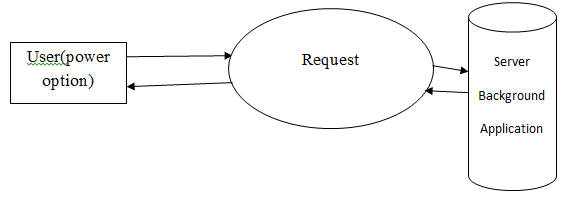
\includegraphics{power1.png}}
{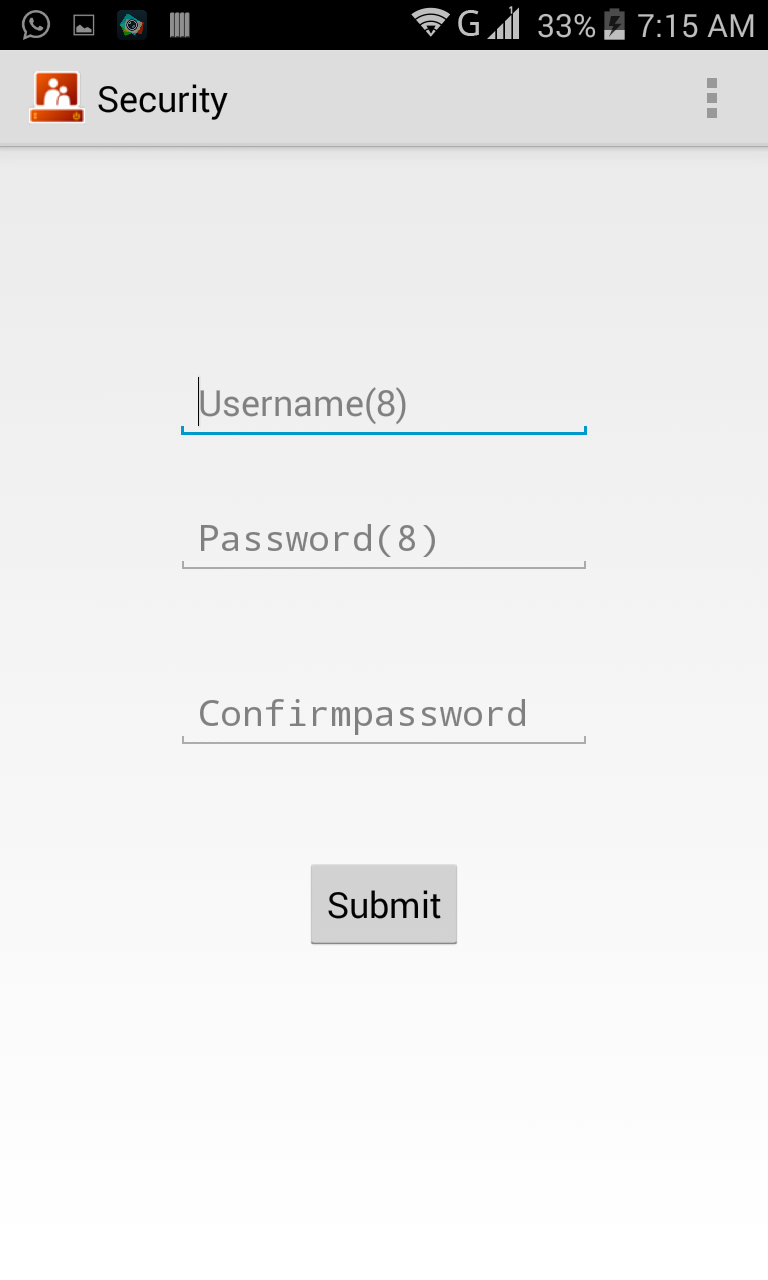
\includegraphics{reg.png}}
\caption{User Registration}  
\end{center}
 The mobile user can register by providing his/her username and password.
\end{figure}
\pagebreak
\begin{figure}
\begin{center}
\scalebox{0.25}
%{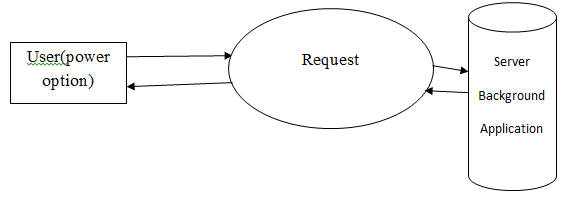
\includegraphics{power1.png}}
{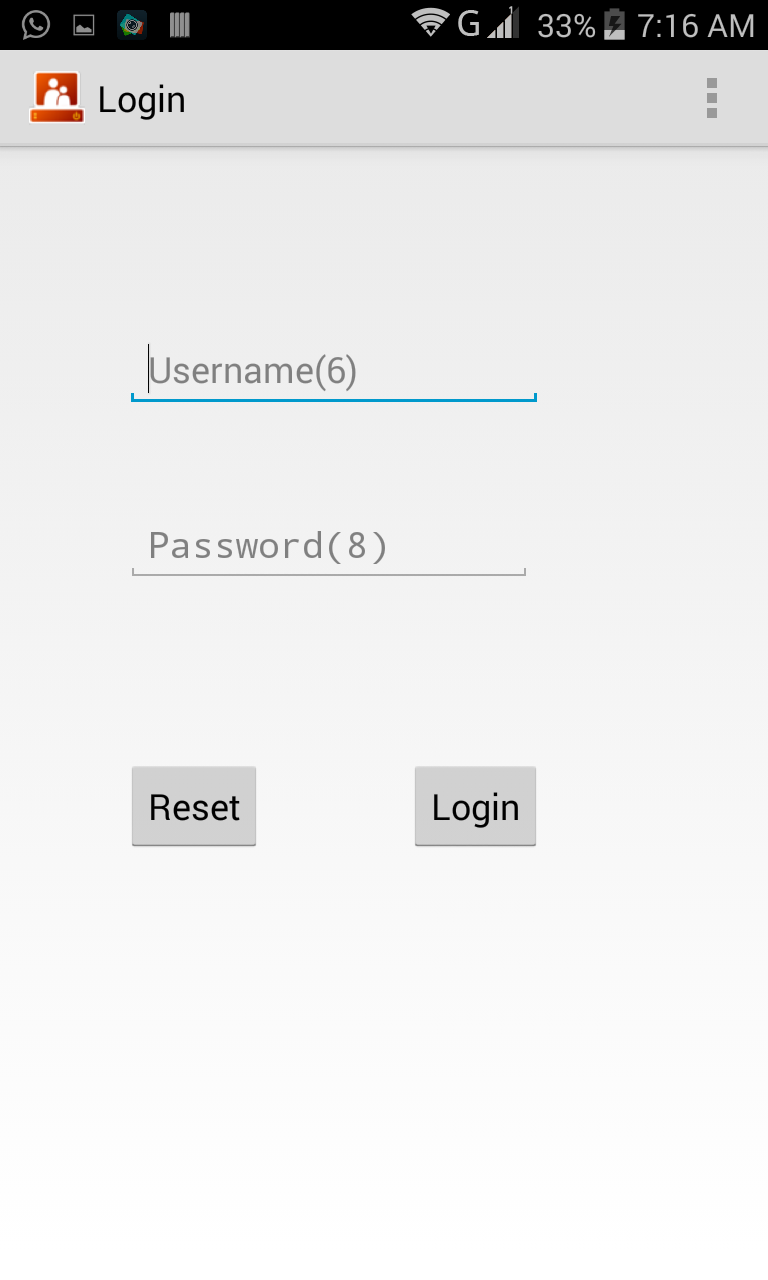
\includegraphics{login.png}}
\caption{User Login}  
\end{center}
The registered user can only login with username and password.
\end{figure}

\begin{figure}
\begin{center}
\scalebox{0.25}
%{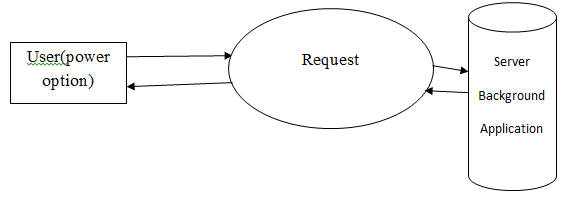
\includegraphics{power1.png}}
{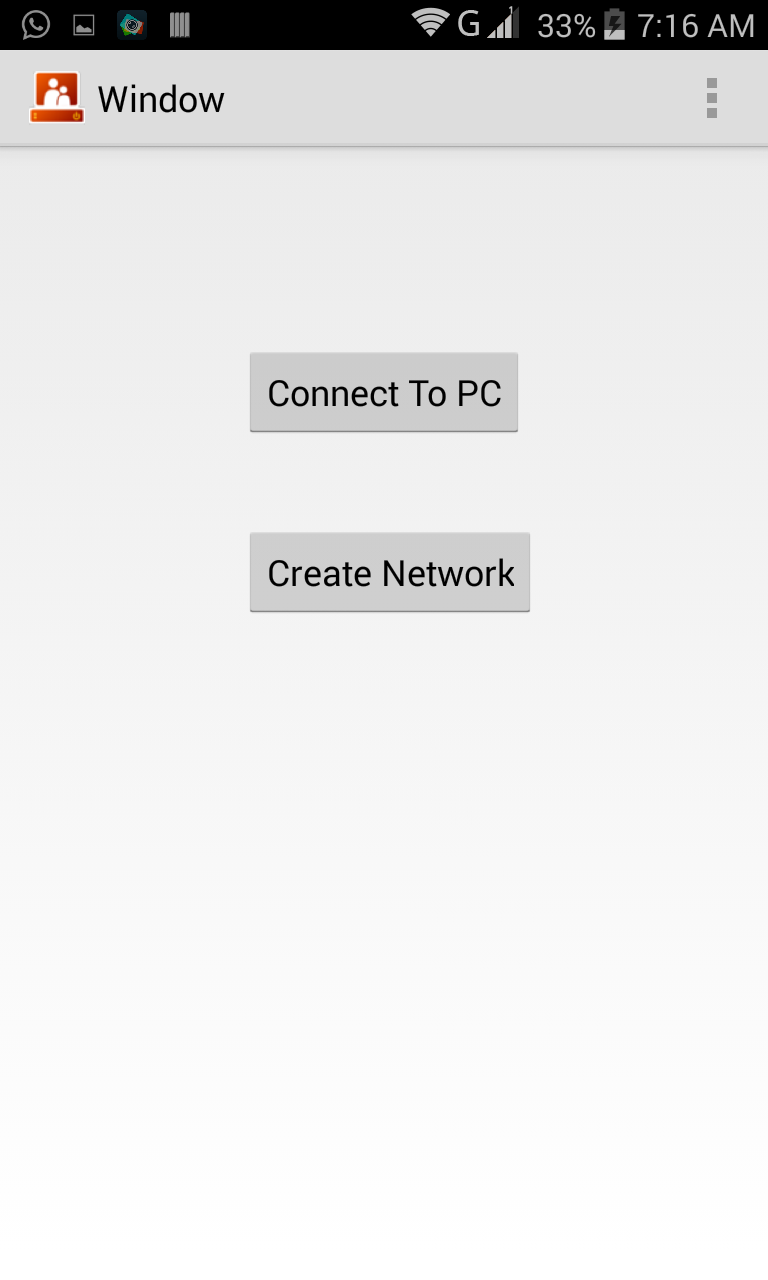
\includegraphics{window.png}}
\caption{Connection Window}  
\end{center}
This window contain two options:'Connect to PC' and 'Create Network'. When Create Network option selected control goes to the settings of android otherwise Connect to PC selected the control goes to the System Configuration. 
\end{figure}

\begin{figure}
\begin{center}
\scalebox{0.25}
%{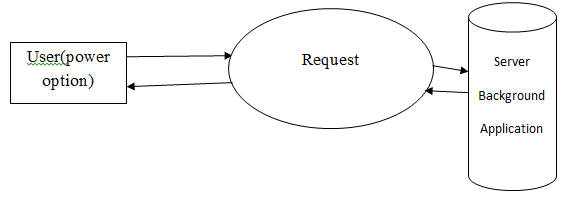
\includegraphics{power1.png}}
{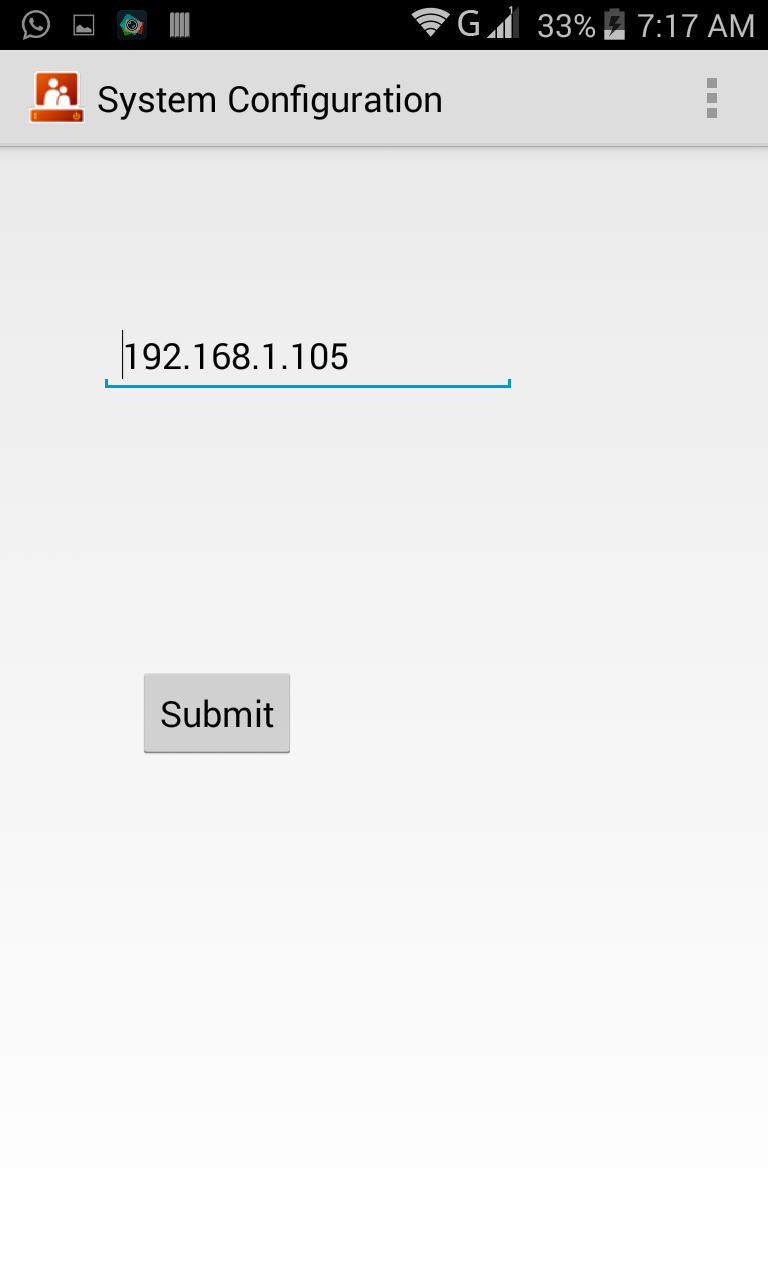
\includegraphics{system.png}}
\caption{System Configuration}  
\end{center}
This window connect the PC to android through IP address. 
\end{figure}

\begin{figure}
\begin{center}
\scalebox{0.25}
%{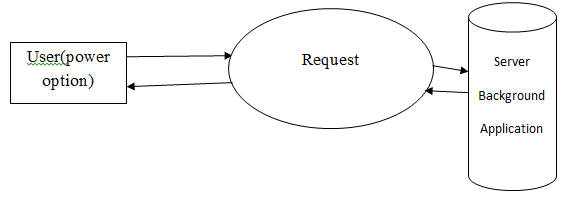
\includegraphics{power1.png}}
{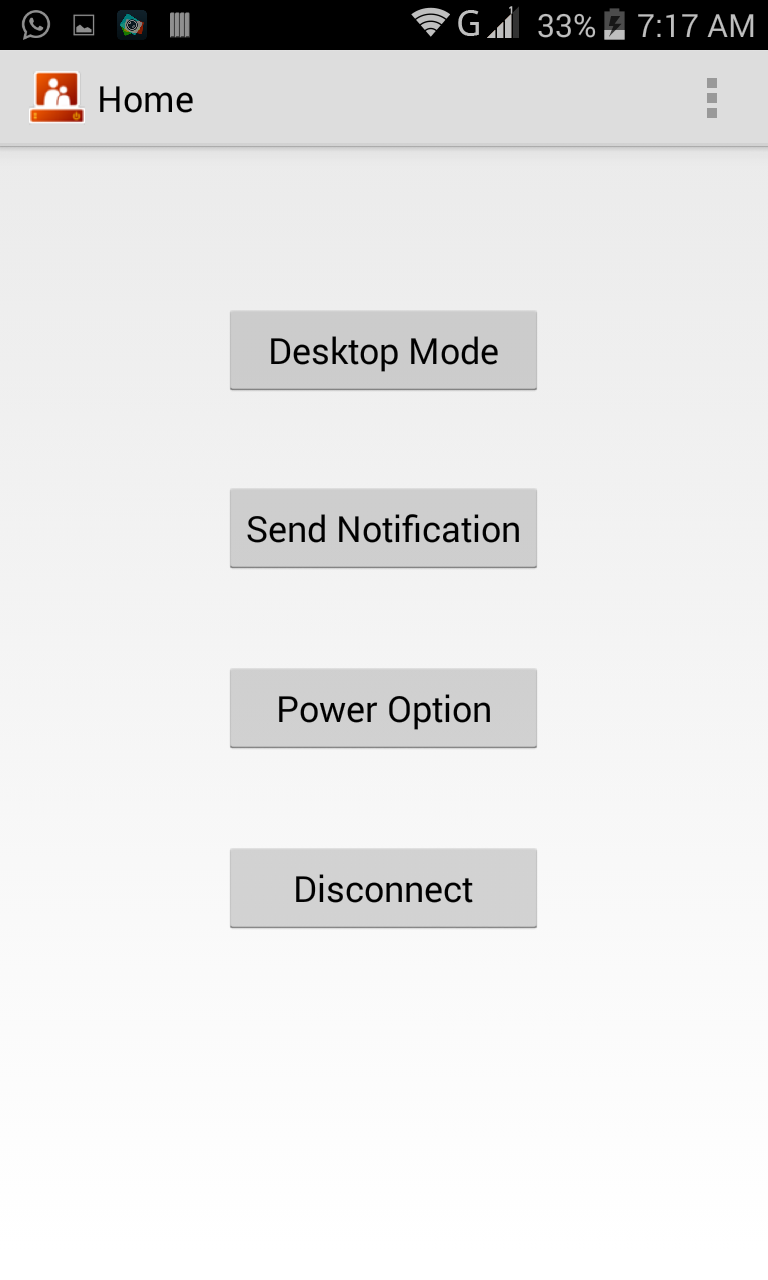
\includegraphics{home.png}}
\caption{Home Options}  
\end{center}
This window contain four selection options:Desktop Mode, Send Notification, Power Options and Disconnect. 
\end{figure}

\begin{figure}
\begin{center}
\scalebox{0.25}
%{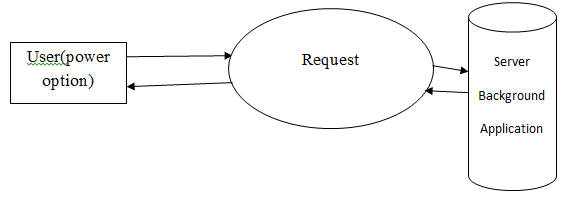
\includegraphics{power1.png}}
{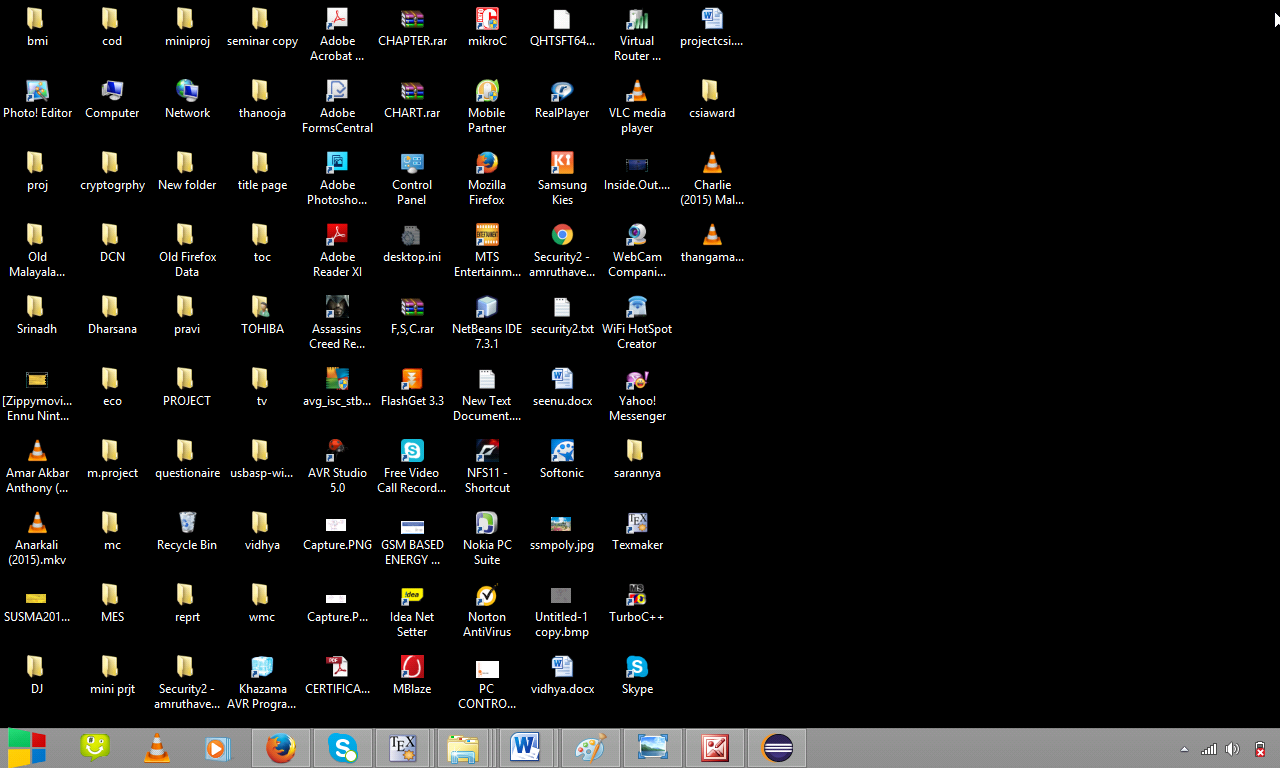
\includegraphics{desk.png}}
\caption{Remote Desktop Access}  
\end{center}
This image shows the remote desktop access of child PC in an android touch screen.
\end{figure}

\begin{figure}
\begin{center}
\scalebox{0.25}
%{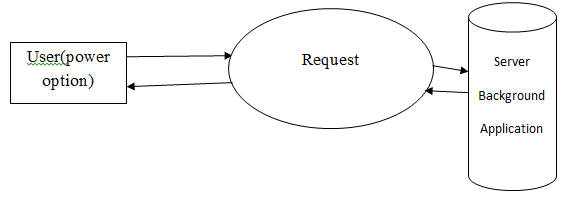
\includegraphics{power1.png}}
{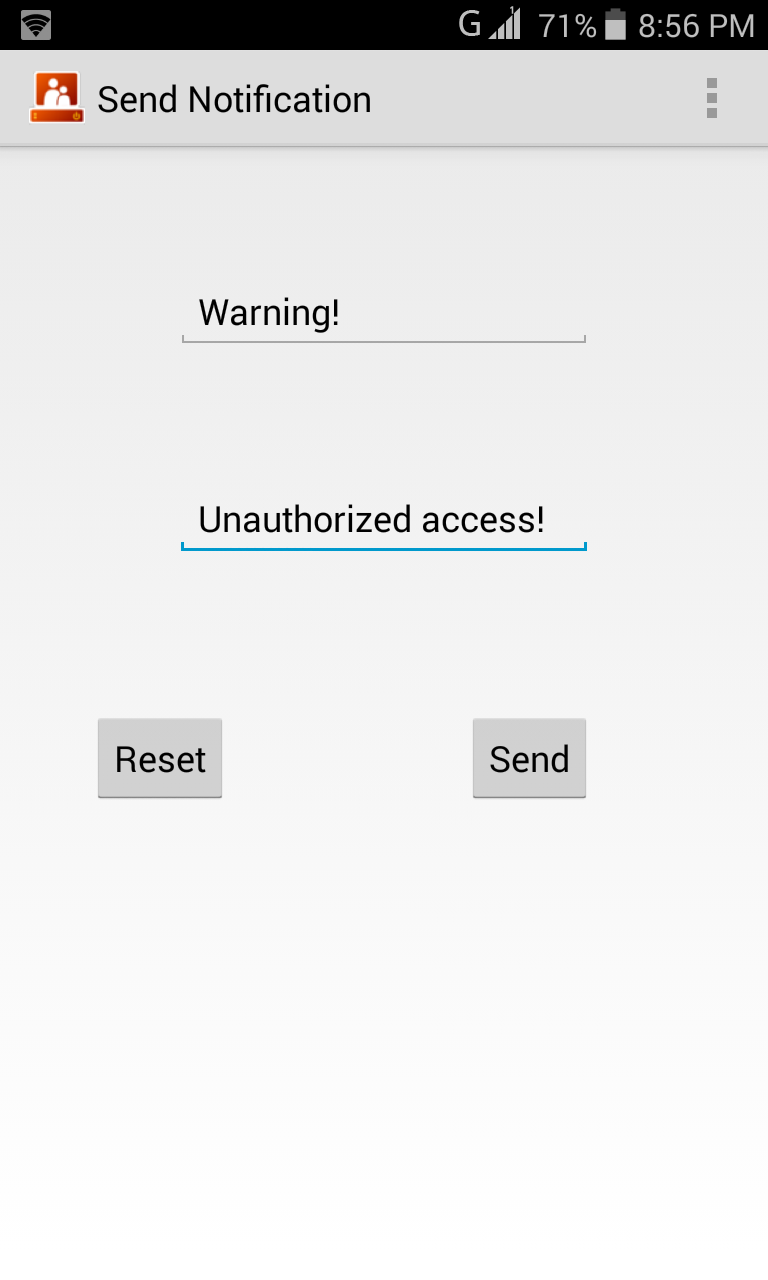
\includegraphics{message.png}}
\caption{Send Notification}  
\end{center}
This window used for send message to remote child PC.
\end{figure}

\begin{figure}
\begin{center}
\scalebox{0.25}
%{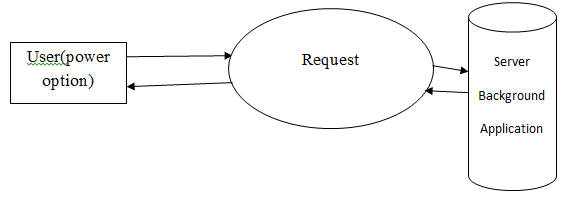
\includegraphics{power1.png}}
{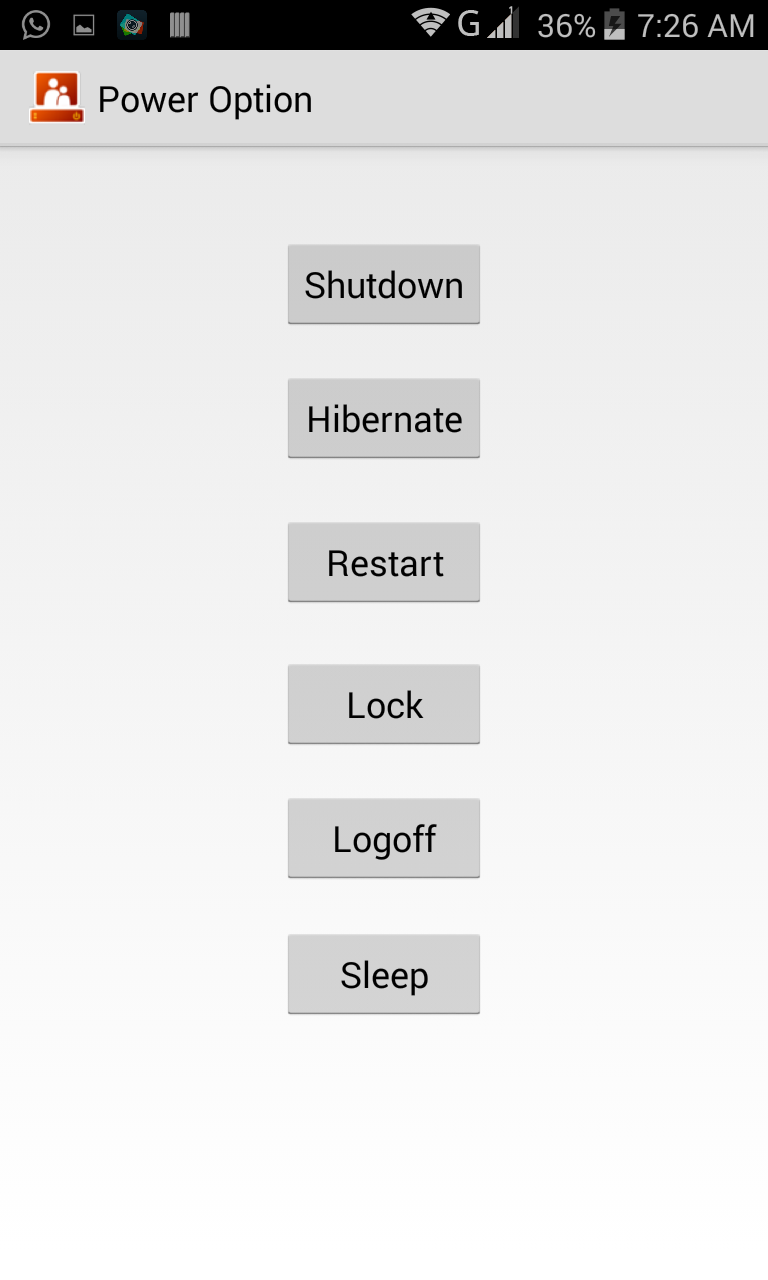
\includegraphics{power.png}}
\caption{Power Options}  
\end{center}
This window used to select shortcuts for power options such as Shutdown, Hibernate, Sleep, Restart, Lock, Logoff etc.   
\end{figure}

\begin{figure}
\begin{center}
\scalebox{0.40}
%{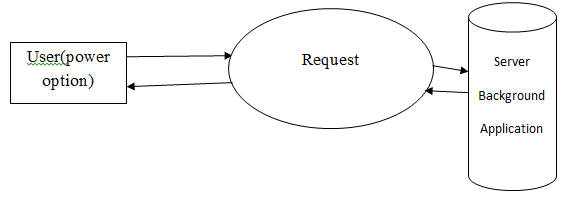
\includegraphics{power1.png}}
{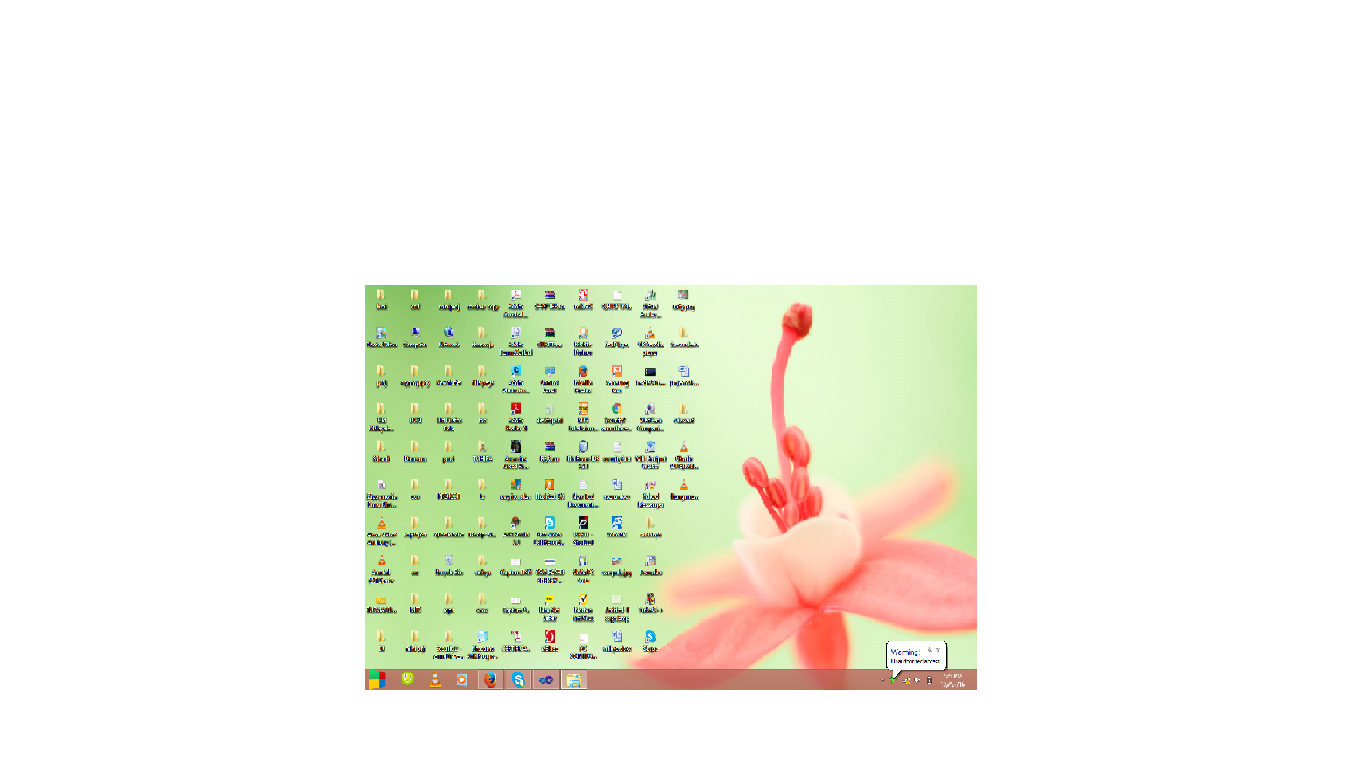
\includegraphics{notify.png}}
\caption{Message Notification}  
\end{center}
This PC desktop image shows the message notification from android.  
\end{figure}


%%%%%%%%%%%%%%%%%%%%%%%%%%%%%%%%%%%%%%%%%%%%%%%%%%%%%%%%%%%%%%%%%%%
%%%%%%%%%%%%%%%%%%%%%%%  Bibliography %%%%%%%%%%%%%%%%%%%%%%%%%%%%%
%%%%%%%%%%%%%%%%%%%%%%%%%%%%%%%%%%%%%%%%%%%%%%%%%%%%%%%%%%%%%%%%%%%

\bibliographystyle{IEEEtran}
% \bibliographystyle{plain}	% or "siam", or "alpha", or "abbrv"
				% see other styles in
				% /usr/local/TeX/texmf/bibtex/bst

\nocite{*}		        % list all refs in database, cited or not.

\bibliography{seminar}		% bib database in "seminar.bib"


\begin{thebibliography}{9}
\bibitem{tvnc} 
	Tristan Richardson, Quentin Stafford-Fraser, Kenneth R. Wood and Andy Hopper, IEEE Internet Computing, vol. 2, no. 1, pp. 83-38, 1998 

\bibitem{t1vnc}

VNC tight encoder-data compression for VNC

K. V. Kaplinsky, Modern Techniques and Technology, 2001. MTT 2001. Proceedings of the 7th International Scientific and Practical Conference of Students, Post-graduates and Young Scientists Year: 2001 Pages:155 - 157, 
DOI: 10.1109/MTT.2001.983781Cited by: Papers (10) | Patents (5)IEEE Conference Publications

\bibitem{iis} 
http://www.iis.net/learn/install/installing-iis
 
\bibitem{vnc} 
 http://tightvnc.com
 
\bibitem{msdn} 
 https://code.msdn.microsoft.com
 
\bibitem{msdn} 
 http://www.vogella.com/tutorials/Eclipse/article.html
 
\bibitem{vb} 
 http://www.vbtutor.net/index.com

\end{thebibliography}



%%%%%%%%%%%%%%%%%%%%%%%%%%%%%%%%%%%%%%%%%%%%%%%%%%%%%%%%%%%%%%%%%%%
%%%%%%%%%%%%%%%%%%%%%%%%  Appendices %%%%%%%%%%%%%%%%%%%%%%%%%%%%%%
%%%%%%%%%%%%%%%%%%%%%%%%%%%%%%%%%%%%%%%%%%%%%%%%%%%%%%%%%%%%%%%%%%%


%%%%%%%%%%%%%%%%%%%%%%%%%%%%%%%%%%%%%%%%%%%%%%%%%%%%%%%%%%%%%%%%%%%
%%%%%%%%%%%%%%%%%%%%%%%%   THE END   %%%%%%%%%%%%%%%%%%%%%%%%%%%%%%
%%%%%%%%%%%%%%%%%%%%%%%%%%%%%%%%%%%%%%%%%%%%%%%%%%%%%%%%%%%%%%%%%%%

\end{document}
